\documentclass[letterpaper]{article}

%----------------------------------------------------------------------
% Packages

\usepackage{amsmath}
\usepackage{amsfonts}
\usepackage{amssymb}
\usepackage{mathtools}
\usepackage{cancel}
\usepackage{graphicx}
\usepackage{xcolor}
\usepackage{tikz, tcolorbox}
\usepackage{siunitx}
\usepackage{geometry}
\usepackage{fancyhdr}
\usepackage{lastpage}
\usepackage{placeins}


%----------------------------------------------------------------------
% Custom Math Commands

% General Shortcuts
\newcommand{\defeq}{\vcentcolon=}  % Define as
\newcommand{\R}{\mathbb{R}}        % Real Numbers
\newcommand{\C}{\mathbb{C}}        % Complex Numbers
\newcommand{\N}{\mathbb{N}}        % Natural Numbers (0, 1, 2, ...)
\newcommand{\Z}{\mathbb{Z}}        % Integers (..., -2, -1, 0, 1, 2, ...)
\newcommand{\Q}{\mathbb{Q}}        % Rational Numbers

% Linear Algebra Shortcuts
\newcommand{\bv}[1]{\boldsymbol{#1}}      % bold vector quantity
\newcommand{\norm}[1]{|| {#1} ||_1}       % generic norm
\newcommand{\onenorm}[1]{|| {#1} ||_1}    % one norm
\newcommand{\twonorm}[1]{|| {#1} ||_2}    % two norm
\newcommand{\infnorm}[1]{|| {#1} ||_\inf} % infinty norm

% Probability and Statistics Shortcuts
\newcommand{\E}[1]{\textrm{E}\left[#1\right]}
\newcommand{\Var}[1]{\textrm{Var}\left(#1\right)}
\newcommand{\Cov}[1]{\textrm{Cov}\left(#1\right)}

% Navigation Shortcuts
\newcommand{\navvec}[3]{\boldsymbol{#1}^{\,#2}_{#3}}              % navigation vector
\newcommand{\navmeas}[3]{\tilde{\boldsymbol{#1}}^{\,#2}_{#3}}     % navigation measurement
\newcommand{\navest}[3]{\hat{\boldsymbol{#1}}^{\,#2}_{#3}}        % navigation estimate
\newcommand{\navC}[2]{C^{\,#1}_{#2}}                              % coordinate frame transformation
\newcommand{\quat}[2]{q^{#1}_{#2}}                                % quaternion

% Misc.
\newcommand{\MATLAB}{MATLAB\,\textsuperscript{\tiny\textregistered}\,}


%----------------------------------------------------------------------
% Begin Document

\begin{document}
	
	
	%------------------------------------------------------------------
	% Title
	
	\title{Homework 1}
	\author{David L. Olson}
	\date{\today}
	
	\maketitle
	
	%------------------------------------------------------------------
	% Table of Contents
	
	\tableofcontents
	
	
	%------------------------------------------------------------------
	% Header and Footer
	
	\thispagestyle{empty}
	\pagestyle{empty}
	
	\fancyhead{}
	\fancyfoot{}
	
	\thispagestyle{fancy}
	\pagestyle{fancy}
	
	\fancyhead[L]{\textbf{Inverse Problems}}
	\fancyhead[R]{\textbf{David L. Olson}}
	
	\fancyfoot[L]{\textbf{Homework 1}}
	\fancyfoot[R]{\thepage\ of \pageref{LastPage}}
	
	
	%------------------------------------------------------------------
	% Begin Technical Content
	
	%----------------------------------------------------------------------
% Problem 1

\begingroup
\allowdisplaybreaks

\newpage
\section{Problem 1}

\textbf{Exercise 2 in Section 3.6}

\subsection{Solution}
	
\textbf{Note: } \textit{My MATLAB code for this homework problem repeats all the steps for example 3.1 so that I can take on this problem. I will only cover the checkerboard test in this write-up.}
\newline

The checkerboard test using $\bv{m}_{true}$ can be reshaped to $\bv{m}_{true} \in \R^9$ such that

\begin{align*}
	\bv{m}_{true} = \begin{bmatrix}
		-1 & 1 & -1 & 1 & -1 & 1 & -1 & 1 & -1
	\end{bmatrix}^T
\end{align*}

which allows for the creation of test data $\bv{d}_{true}$ and a recovered model $\bv{m}_{\dagger}$.

\begin{align*}
	\bv{d}_{true} &= G \bv{m}_{true} \\
	\\
	\bv{m}_{\dagger} &= G^{\dagger} \bv{d}_{true}
\end{align*}

Recall from example 3.1 that $G \in \R^{8 \times 9}$ with rank $7$. Therefore the generalized pseudo-inverse of $G$, represented as $G^{\dagger}$, was computed using the Moore-Penrose pseudo-inverse function \verb*|pinv(G)| in \MATLAB. Figure \ref{fig: prob1 checkerboard test} shows how the recovered model compares to the true model. 

\begin{figure}[h] 
	\centering
	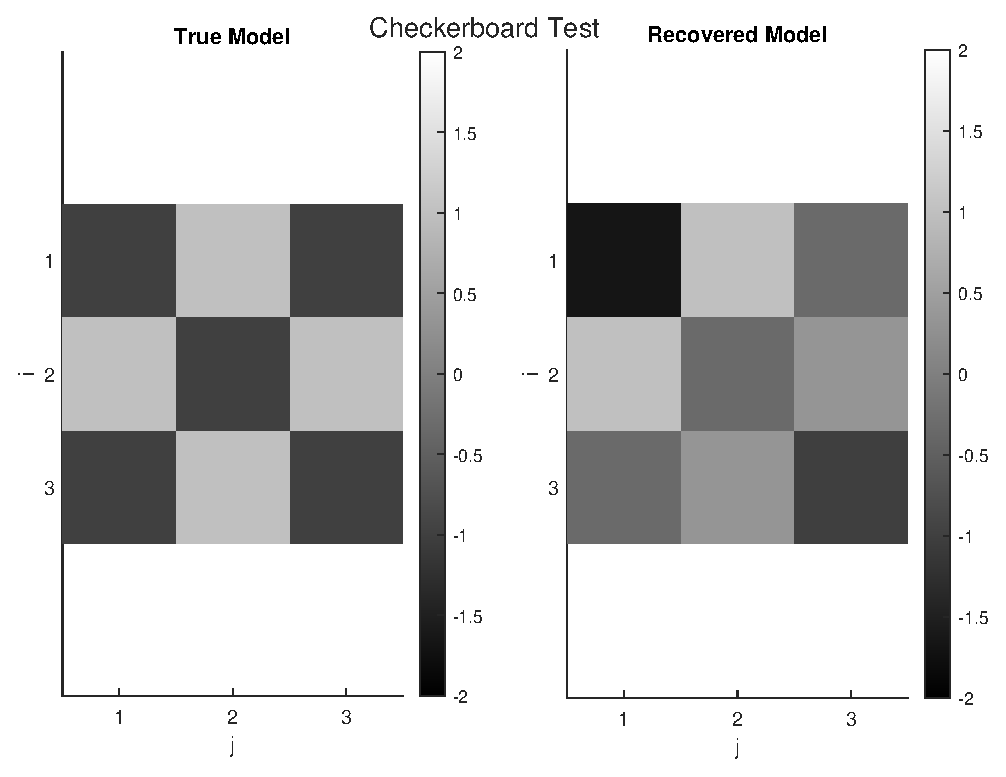
\includegraphics[width=0.85\textwidth]{./images/prob1_checkerboard_test.eps}
	\caption{Checkerboard Test}
	\label{fig: prob1 checkerboard test}
\end{figure}
\FloatBarrier

Recall that this problem is of the situation "$p < m$ and $p < n$", in which both the model and data null spaces are non-trivial and $\bv{m}_\dagger$ is the minimum length solution. The resulting model null space vector, $\bv{m}_0 \defeq \bv{m}_{true} - \bv{m}_{\dagger}$, is shown below both numerically and graphically in figure \ref{fig: prob1 model null space vector}.

\begin{align*}
	\bv{m}_0 = \begin{bmatrix}
		\frac{2}{3} & 0 & \frac{-2}{3} & 0 & \frac{-2}{3} & \frac{2}{3} & \frac{-2}{3} & \frac{2}{3} & 0
	\end{bmatrix}^T
\end{align*}

\begin{figure}[h] 
	\centering
	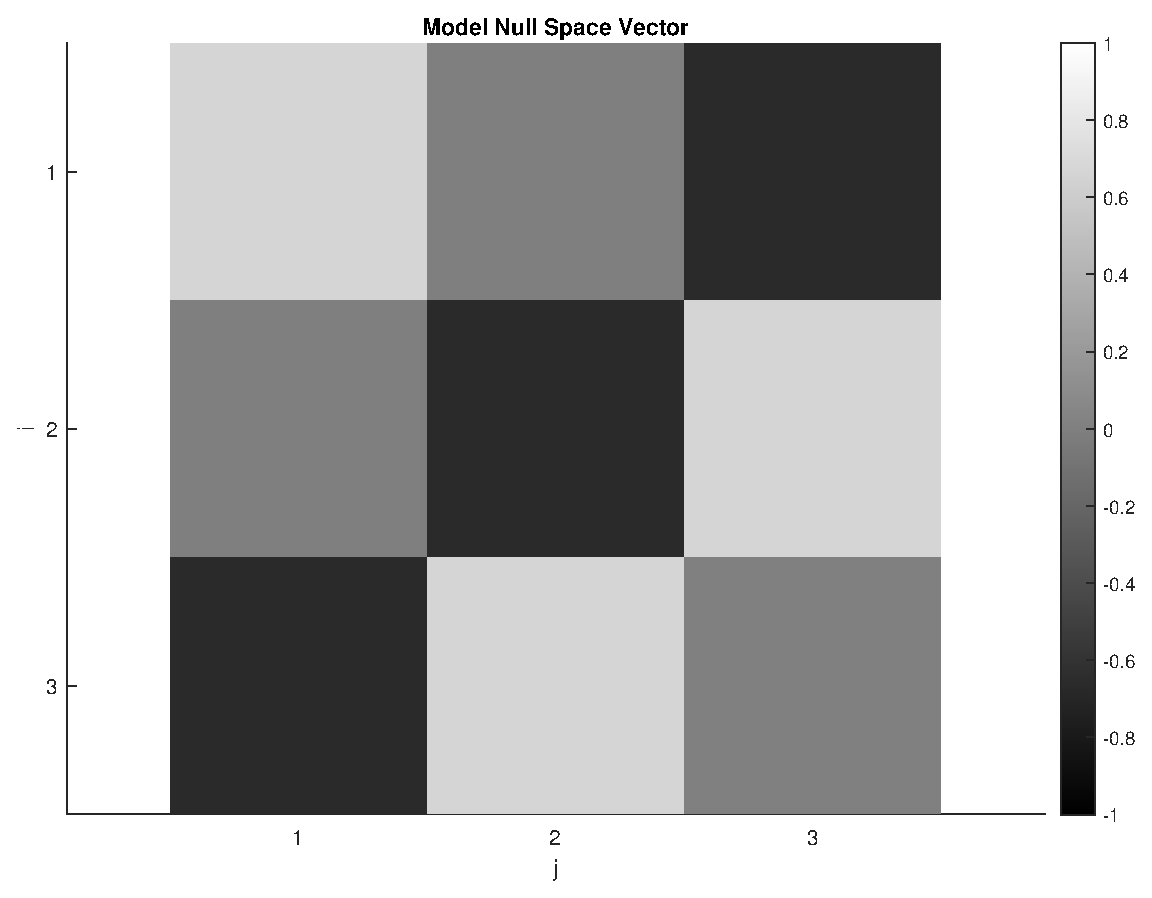
\includegraphics[width=0.85\textwidth]{./images/prob1_model_null_space_vector.eps}
	\caption{Model Null Space Vector}
	\label{fig: prob1 model null space vector}
\end{figure}
\FloatBarrier

Notice that the sum of the model null space vector is zero. Also notice that all of the rows and columns depicted in figure \ref{fig: prob1 model null space vector} also sum to zero. The model null space vector, a.k.a. the model residual, could be restated as

\begin{align*}
	\bv{m}_0 = \sum_{i = p + 1}^{n} \alpha_i V_{.,i}
\end{align*}

where non-zero coefficients for $\alpha_i$ could create other model null space vectors. In our case we computed the minimum length solution, implying that all $\alpha_i$ coefficients are zero. The addition of this vector which resides in the model null space would have no impact on the predicted data if added to another model solution which resides in the model range space.

The three perfectly recovered model parameters are $m_2,\,m_4$ and $m_9$. When examining the model resolution matrix $R_m$ from the spike test, model parameter $m_9$ is the only parameter with perfect resolution. 

\begin{figure}[h] 
	\centering
	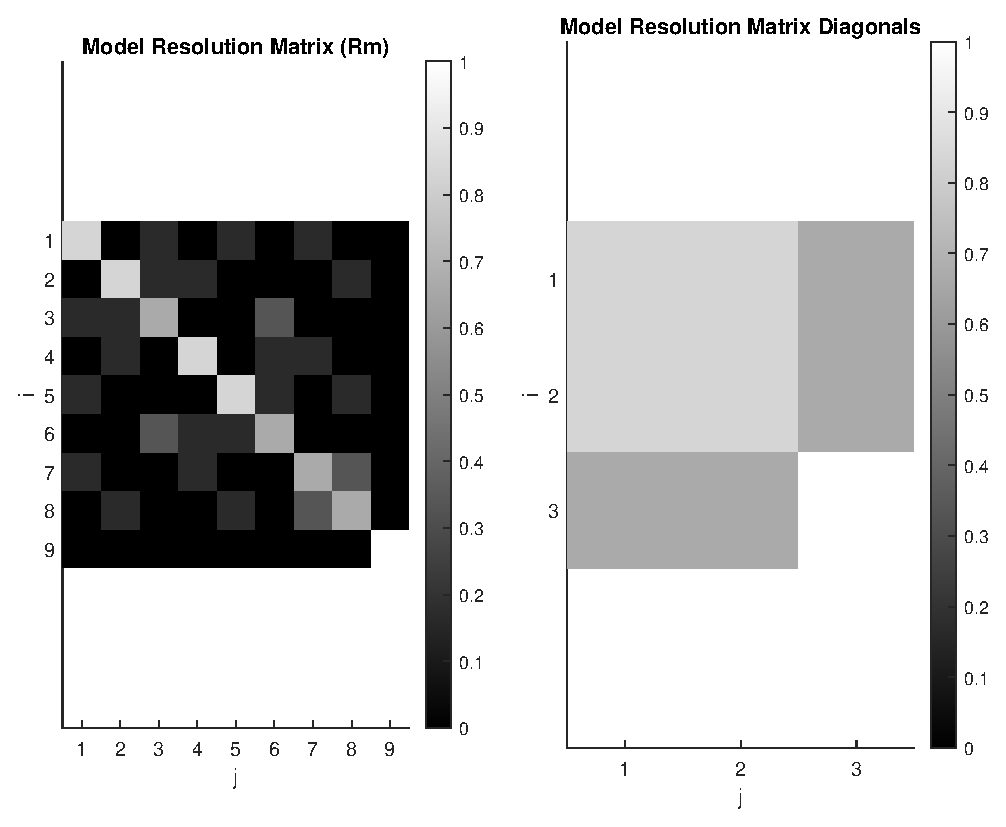
\includegraphics[width=0.85\textwidth]{./images/prob1_Rm.eps}
	\caption{Checkerboard Test}
	\label{fig: prob1 Rm}
\end{figure}
\FloatBarrier

Model parameters $m_2,\,m_4$ are subject to "smearing" due to the limited resolution. In this situation, this could have caused us to assume that model parameters $m_2,\,m_4$ also have perfect resolution, when instead the smearing for the parameters just happened to bring these model parameters to zero.


	
	%----------------------------------------------------------------------
% Problem 2

\begingroup
\allowdisplaybreaks

\newpage
\section{Problem 2}

\textbf{Exercise 8 in Section 9.6}

\subsection{Solution}


	
	%----------------------------------------------------------------------
% Problem 3

\begingroup
\allowdisplaybreaks

\newpage
\section*{Problem 3}

\begin{figure}[h]
	\centering
	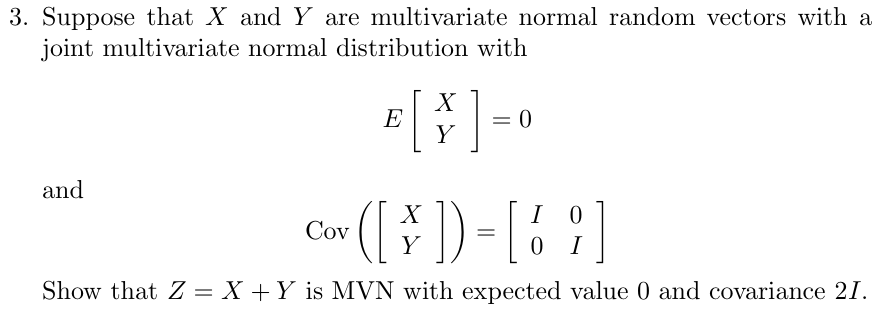
\includegraphics[width=0.8\textwidth]{./images/prob3_statement.png}
\end{figure}

\subsection*{Solution}

Given the problem statement, let random vectors $\bv{X}$ and $\bv{Y}$ be of equal dimension such that

\begin{align*}
	\bv{X},\,\bv{Y} \sim \textrm{N}\left(0,\,I\right)
\end{align*}

Creating a new random vector $\bv{Z} = \bv{X} + \bv{Y}$, the expected value of $\bv{Z}$ is

\begin{align*}
	\E{\bv{Z}} &= \E{\bv{X} + \bv{Y}} \\
	\\
	&= \E{\bv{X}} + \E{\bv{Y}} \\
	\\
	&= \bv{0} + \bv{0} \\
	\\
	&= \bv{0} \,\,\,\,\, \textcolor{green}{\checkmark}
\end{align*}

To determine the covariance of $\bv{Z}$, we must first find a matrix $A$ such that $\bv{Z} = \bv{X} + \bv{Y}$. $A$ is defined as:

\begin{align*}
	\bv{Z} &= A \begin{bmatrix} \bv{X} \\ \bv{Y} \end{bmatrix}
	\\
	\bv{Z} &= \begin{bmatrix} I & I \end{bmatrix} \begin{bmatrix} \bv{X} \\ \bv{Y} \end{bmatrix}
	\\
	\\
	\\
	A &\defeq \begin{bmatrix} I & I \end{bmatrix}
\end{align*}

The covariance of $\bv{Z}$ is given by the transformation $\bv{Z} = A C A^T$, which is shown below.

\begin{align*}
	\Cov{\bv{Z}} &= A \Cov{\begin{bmatrix} \bv{X} \\ \bv{Y} \end{bmatrix}} A^T \\
	\\
	&= \begin{bmatrix} I & I \end{bmatrix} \begin{bmatrix} I & 0 \\ 0 & I \end{bmatrix} \begin{bmatrix} I \\ I \end{bmatrix} \\
	\\
	&= \begin{bmatrix} I & I \end{bmatrix} \begin{bmatrix} I \\ I \end{bmatrix} \\
	\\
	&= I + I \\
	\\
	&= 2I \,\,\,\,\, \textcolor{green}{\checkmark}
\end{align*}


	
	%----------------------------------------------------------------------
% Problem 4

\begingroup
\allowdisplaybreaks

\newpage
\section{Problem 4}

\textbf{Exercise 5 in Section 4.10}

\subsection{Solution}

To bias a model solution towards a particular solution $\bv{m}_0$, the objective function can be modified to be expressed accordingly below.

\begin{align*}
	\textrm{min} \twonorm{G \bv{m} - \bv{d}}^2 + \alpha^2 \twonorm{L \left(\bv{m} - \bv{m}_0 \right) }^2
\end{align*}

The expression within the minimization is a function of $f \left( \bv{m} \right)$ which can be expanded.

\begin{align*}
	f \left( \bv{m} \right) &= \twonorm{G \bv{m} - \bv{d}}^2 + \alpha^2 \twonorm{L \left(\bv{m} - \bv{m}_0 \right) }^2 \\
	\\
	&= \left(G \bv{m} - \bv{d} \right)^T \left(G \bv{m} - \bv{d} \right) + \alpha^2 \left( \left( L \bv{m} - L \bv{m}_0 \right)^T \left( L \bv{m} - L \bv{m}_0 \right) \right) \\
	\\
	&= \left(\bv{m}^T G^T - \bv{d}^T \right) \left(G \bv{m} - \bv{d} \right) + \alpha^2 \left( \left( \bv{m}^T L^T - \bv{m}_0^T L^T \right) \left( L \bv{m} - L \bv{m}_0 \right) \right) \\
	\\
	&= \bv{m}^T G^T G \bv{m} - \bv{m}^T G^T \bv{d} - \bv{d}^T G \bv{m} + \bv{d}^T \bv{d} + \alpha^2 \left( \bv{m}^T L^T L \bv{m} - \bv{m}^T L^T L \bv{m}_0 - \bv{m}_0^T L^T L \bv{m} + \bv{m}_0^T L^T L \bv{m}_0 \right)
\end{align*}

Notice that terms $\bv{m}^T G^T \bv{d}$ and $\bv{d}^T G \bv{m}$ both evaluate to the same scalar value which means the can be added together to the term $2 \bv{m}^T G^T \bv{d}$. \textcolor{red}{Can the same be said for the other terms?... let's assume they do for now...}

\begin{align*}
	f \left( \bv{m} \right) &= \bv{m}^T G^T G \bv{m} - 2 \bv{m}^T G^T \bv{d} \bv{d}^T \bv{d} + \alpha^2 \left( \bv{m}^T L^T L \bv{m} - 2 \bv{m}_0^T L^T L \bv{m} + \bv{m}_0^T L^T L \bv{m}_0 \right) \\
	\\
	&= \bv{m}^T G^T G \bv{m} - 2 \bv{m}^T G^T \bv{d} + \bv{d}^T \bv{d} + \alpha^2 \bv{m}^T L^T L \bv{m} - 2 \alpha^2 \bv{m}_0^T L^T L \bv{m} + \alpha^2 \bv{m}_0^T L^T L \bv{m}_0
\end{align*}

To solve for the minimum, we must set the gradient of $\nabla f \left( \bv{m} \right) = \bv{0}$. This leads to the following expression below. 

\begin{align*}
	\nabla f \left( \bv{m} \right) = 2 G^T G \bv{m} - 2 G^T \bv{d} + 2 \alpha^2 L^T L \bv{m} - 2 \alpha^2 L^T L \bv{m}_0 = \bv{0} \\
	\\
	G^T G \bv{m} + \alpha^2 L^T L \bv{m} &= G^T \bv{d} + \alpha^2 L^T L \bv{m}_0
\end{align*}

This expression can be expanded into matrix form resulting in a linear system of equations. 

\begin{align*}
	\begin{bmatrix} G^T & \alpha L^T \end{bmatrix} \begin{bmatrix} G \\ \alpha L \end{bmatrix} \bv{m} = \begin{bmatrix} G^T & \alpha^2 L^T L \end{bmatrix} \begin{bmatrix} \bv{d} \\ \bv{m}_0 \end{bmatrix}
\end{align*}

The normal equations and model solution are also expressed as:

\begin{align*}
	\left(G^T G + \alpha^2 L^T L \right) \bv{m} &= G^T \bv{d} + \alpha^2 L^T L \bv{m}_0 \\
	\\
	\bv{m} &= \left(G^T G + \alpha^2 L^T L \right)^{-1} \left( G^T \bv{d} + \alpha^2 L^T L \bv{m}_0 \right)
\end{align*}



\end{document}


%----------------------------------------------------------------------
% Additional Copy-and-Paste Templates

% Figure

%\begin{figure}[h] \label{fig: my figure}
%	\centering
%	\includegraphics[width=0.8\textwidth]{./images/<image.png>}
%	\caption{\textcolor{red}{provide a caption}}
%\end{figure}


% Table

%\begin{center}
%	\begin{tabular} { | h1 | h2 | h3 | } \label{tab: my table}
%		
%		\hline
%		x11 & x12 & x13 \\
%		\hline
%		x21 & x22 & x23 \\
%		\hline
%		x31 & x32 & x33 \\
%		\hline
%		
%	\end{tabular}
%	\caption{\textcolor{red}{put caption here}
%\end{center}








